%%%%%%%%%%%%%%%%%%%%%%%%%%%%%%%%%%%%%%%%%%%%%%%%%%%%%%%%%%%%%%%%%%%%%%%%%%%%%%%
% Definici�n del tipo de documento.                                           %
% Posibles tipos de papel: a4paper, letterpaper, legalpapper                  %
% Posibles tama�os de letra: 10pt, 11pt, 12pt                                 %
% Posibles clases de documentos: article, report, book, slides                %
%%%%%%%%%%%%%%%%%%%%%%%%%%%%%%%%%%%%%%%%%%%%%%%%%%%%%%%%%%%%%%%%%%%%%%%%%%%%%%%
\documentclass[a4paper,10pt]{article}


%%%%%%%%%%%%%%%%%%%%%%%%%%%%%%%%%%%%%%%%%%%%%%%%%%%%%%%%%%%%%%%%%%%%%%%%%%%%%%%
% Los paquetes permiten ampliar las capacidades de LaTeX.                     %
%%%%%%%%%%%%%%%%%%%%%%%%%%%%%%%%%%%%%%%%%%%%%%%%%%%%%%%%%%%%%%%%%%%%%%%%%%%%%%%

% Paquete para inclusi�n de gr�ficos.
\usepackage{graphicx}

% Paquete para definir la codificaci�n del conjunto de caracteres usado
% (latin1 es ISO 8859-1).
\usepackage[latin1]{inputenc}

% Paquete para definir el idioma usado.
\usepackage[spanish]{babel}

% T�tulo principal del documento.
\title{\textbf{Trabajo pr\'actico 2:\\ Arquitecturas de memoria}}

% Informaci�n sobre los autores.
\author{Roberto Herman, \textit{Padr\'on Nro. 84.803}\\
            \texttt{ berta1108@gmail.com }\\
            Mat\'ias Waisgold, \textit{Padr\'on Nro. 88.464}\\
            \texttt{ mwaisgold@gmail.com }\\
            Nicol\'as Suarez, \textit{Padr\'on Nro. 83.752}\\
            \texttt{ nicolas.suarez@gmail.com }\\
            Federico Rodriguez, \textit{Padr\'on Nro. 88.310}\\
            \texttt{ fede1726@gmail.com }\\[2.5ex]
            \normalsize{2do. Cuatrimestre de 2009}\\
            \normalsize{66.20 Organizaci\'on de Computadoras}\\
            \normalsize{Facultad de Ingenier\'ia, Universidad de Buenos Aires}\\
       }
\date{}



\begin{document}

% Inserta el t�tulo.
\maketitle

% Quita el n�mero en la primer p�gina.
\thispagestyle{empty}

\newpage

\section{Introducci\'on}

El presente trabajo pr\'actico pretende familiarizar al alumno con el uso de herramientas de profiling.
El objetivo del trabajo ser\'a determinar el tama\~no de bloque, la cantidad de vias y el tama\~no total
de una memoria cache L1 de datos.\\
Utilizaremos el m\'odulo Cachegrind de la herramienta Valgrind\cite{Valgrind}, que nos permite simular diferentes memorias
cache y obtener las tasas de misses a partir de las cuales podremos determinar los datos de la cache.

\section{Dise\~no e implementaci\'on}

\subsection{M\'odulo principal}
El m\'odulo principal se encarga de ejecutar cada uno de los m\'odulos y obtener la tasa de misses para realizar
el c\'alculo de la cache.

\subsection{Tama\~no del Bloque}
Para el c\'alculo del tama\~no del bloque se ejecuta el m\'odulo \textit{tamanioBloque}. Este m\'odulo realiza un lazo
escribiendo un array de tama\~no 1024 KB. Al finalizar el lazo habremos accedido a todos los bloques de la cache, por lo cual obteniendo la cantidad de accesos por escritura (dw) y la tasa de misses de escritura (d1mw) de la cache, podemos caclular el tama\~no del bloque haciendo el siguiente c\'alculo:
\begin{center}
sizeBloque = dw/d1mw.
\end{center}

\subsection{Tama\~no total de la Cache}
Para el c\'alculo del tama\~no total de la cache lo que hacemos es determinar la cantidad total de bloques, luego multiplicando
esa cantidad por el tama\~no del bloque obtenemos el tama\~no de la cache.\\
Para calcular la cantidad de bloques ejecutamos el m\'odulo \textit{tamanioCache}. Este m\'odulo recibe dos par\'ametros: el tama\~no del bloque (\textit{sizeBloque}) y un valor \textit{n} que es la cantidad hipot\'etica de bloques de la cache. El m\'odulo realiza un lazo dos veces escribiendo un array cuyo tama\~no es \textit{sizeBloque*n}.\\
Luego de ejecutar el m\'odulo se obtiene la taza de misses de escritura, si esa cantidad es menor o igual a \textit{n} no se ha recorrido todos los bloques por lo cual se vuelve a ejecutar el m\'odulo duplicando el valor de \textit{n}.

\subsection{Cantidad de vias}
Para determinar la cantidad de vias lo que hacemos es recorrer un lazo de una matriz de char, la cual tendr\'a tantas columnas como el tama\~no de la cache y tantas filas como la cantidad de vias que suponemos que tiene (inicialmente una).\\
Al finalizar el lazo, volvemos a acceder a las dos primeras posiciones de cada una de las filas de la matriz, es decir que estariamos accediendo al primer bloque de cada via. Si en los dos \'ultimos accesos se producen misses en la cache quiere decir que hemos accedido a todos los bloques de cada una de las vias, sino la cantidad de vias es mayor, por lo cual duplicamos el valor la cantidad de vias y volvemos a ejecutar el lazo.

\section{Compilaci\'on del benchmark}
Para compilar el benchmark se debe correr el makefile.\\
Desde la consola se debe entrar al directorio donde se encuentran el codigo fuente y el makefile, y luego ejecutar el comando \textit{make}:
\begin{verbatim}
$> make
\end{verbatim}
Al finalizar la compilaci\'on se habr\'an generado cuatro archivos ejecutables:\\
\begin{itemize}
 \item tp2 (Este es el programa principal)
 \item tamanioBloque
 \item tamanioCache
 \item cantidadVias
\end{itemize}

\section{Instrucciones de uso}
El benchmark se puede utilizar sobre una cache simulada o sobre la cache propia de la maquina que se est\'e utilizando.\\
\begin{itemize}
\item 
Para el caso de una cache simulada se debe pasar como par\'ametro el tama\~no de total, la cantidad de vias y tama\~no del bloque de la cache a simular. Por ejemplo, para correr el benchmark sobre una cache simulada de 2 vias, con tama\~no de bloque de 32 bytes y tama\~no total de 32768 bytes:
\begin{verbatim}
$>./tp2 --D1=32768,2,32
\end{verbatim}

\item 
Para el segundo caso simplemente debemos ejecutar el programa sin par\'ametros:
\begin{verbatim}
$>./tp2
\end{verbatim}

\end{itemize}

\newpage

\section{Corridas de prueba}
\begin{itemize}
	\item Prueba 1: Simulando una cache de 32.768 bytes, 4 vias, 32 bytes de l\'inea.
	\begin{figure}[h]
	\centering
	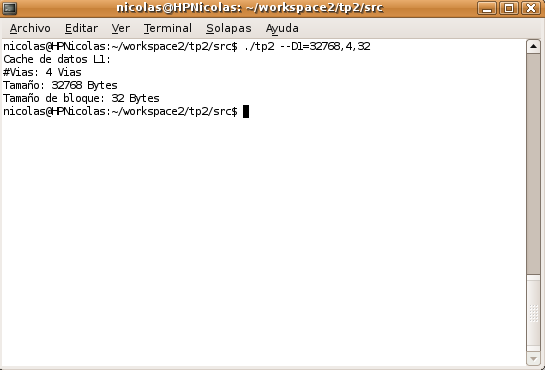
\includegraphics[width=0.8\textwidth]{Prueba1.png}
	\caption{./tp2 --D1==32768,4,32}
	\end{figure}

	\item Prueba 2: Simulando una cache Full Asociative de 8.192 bytes y 32 bytes de l\'inea.
	\begin{figure}[h]
	\centering
	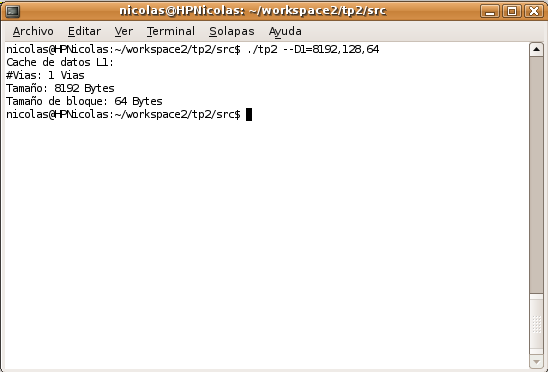
\includegraphics[width=0.8\textwidth]{Prueba2.png}
	\caption{./tp2 --D1==8192,128,64}
	\end{figure}
\end{itemize}

\begin{itemize}
	\newpage

	\item Prueba 3: Sin simular cache.
	\begin{figure}[h]
	\centering
	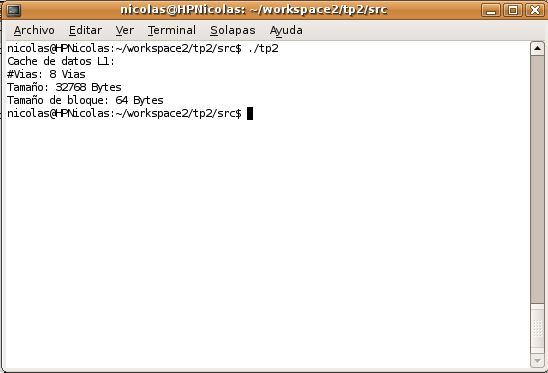
\includegraphics[width=0.8\textwidth]{Prueba3.png}
	\caption{./tp2}
	\end{figure}

	\item Prueba 4: Cache Direct Mapped, 16Bytes de l\'inea, 8Kb tama\~no total
	\begin{figure}[h]
	\centering
	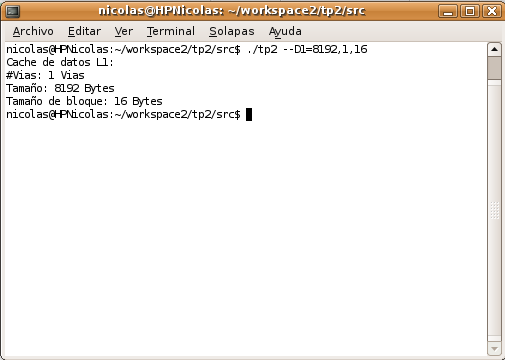
\includegraphics[width=0.8\textwidth]{Prueba4.png}
	\caption{./tp2 --D1=8192,1,16}
	\end{figure}
\end{itemize}

\newpage

\section{Conclusiones}
El trabajo pr\'actico nos permiti\'o conocer las caracter\'istacas y funcionamiento de la memoria cache. A su vez nos hemos familiarizado con la herramienta de profiling Valgrind, la cual nos permite saber, al correr una aplicaci\'ion, en que partes de esta se esta accediendo a la memoria cache y obtener la tasa de misses, y en base a esta informaci\'on podemos mejorar la aplicaci\'on para obtener un mayor rendimiento.

% Citas bibliogr�ficas.
\begin{thebibliography}{99}

\bibitem{Valgrind}
Valgrind: http://valgrind.org/
\end{thebibliography}

\newpage

\appendix

\section{Ap\'endice: C\'odigo Fuente}

\subsection{M\'odulo Principal: tp2.cpp}
\begin{verbatim}
#include <iostream>
#include <string>
#include <fstream>
#include <sstream>
#include <stdlib.h>
#include <stdio.h>
#include <string.h>
#include <getopt.h>

#define TAMANIO_BLOQUE "tamanioBloque"
#define TAMANIO_CACHE "tamanioCache"
#define CANT_VIAS "cantidadVias"
#define CACHEGRIND  "valgrind --tool=cachegrind --log-file=salidaValgrind
                      --cachegrind-out-file=salidaCachegrind "
#define CG_ANNOTATE "cg_annotate --auto=yes --show=Dr,Dw,D1mr,D1mw salidaCachegrind "
#define FILE_OUTPUT_CACHEGRIND "salidaCachegrind"
#define FILE_OUTPUT_CGANNOTATE "salidaCgannotate"
#define FILE_OUTPUT_GREP "salidaGrep"
#define FILE_OUTPUT_VALGRIND "salidaValgrind"
#define SIZE_BUFFER 512

using std::string;

void imprime_uso (FILE *output)
{
    fprintf(output, "Usage:\n");
    fprintf(output, "    tp2 -h\n"
           "    tp2 -V\n"
           "    tp2 [Cache data]\n"
           "Options:\n"
           "    -h, --help    Imprime ayuda.\n"
           "    -V, --version   Version del programa.\n"
           "Examples:\n"
           "    tp2 --D1=16384,2,64\n");
}

void imprime_version()
{
    printf("Version [66.20] Organizacion de Computadoras\n"
           "Segundo Cuatrimestre 2009\n");
}

bool datosCacheValidos(char* datos)
{
    int i= 5;
    char c;

    c= datos[i];
    while(c != ','){
        if(c == '\0')
            return false;

        if((c == '0') || (c == '1') || (c == '2') ||
           (c == '3') || (c == '4') || (c == '5') ||
           (c == '6') || (c == '7') || (c == '8') || (c == '9'))
        {
            i++;
            c= datos[i];
        }
        else{
            return false;
        }

    }

    i++;
    c= datos[i];

    while(c != ','){
        if(c == '\0')
            return false;

        if((c == '0') || (c == '1') || (c == '2') ||
           (c == '3') || (c == '4') || (c == '5') ||
           (c == '6') || (c == '7') || (c == '8') || (c == '9'))
        {
            i++;
            c= datos[i];
        }
        else{
            return false;
        }
    }

    i++;
    c= datos[i];

    if((c == '0') || (c == '1') || (c == '2') ||
       (c == '3') || (c == '4') || (c == '5') || 
       (c == '6') || (c == '7') || (c == '8') || (c == '9'))
    {
        i++;
        c= datos[i];
    }
    else{
        return false;
    }

    while(c != '\0'){
        if((c == '0') || (c == '1') || (c == '2') ||
           (c == '3') || (c == '4') || (c == '5') ||
           (c == '6') || (c == '7') || (c == '8') || (c == '9'))
        {
            i++;
            c= datos[i];
        }
        else{;
            return false;
        }
    }

    return true;
}

void replaceText(string &word, const string &toReplace, const string &replaceBy)
{

    string::size_type posToRepleace = word.find(toReplace);
    while(posToRepleace != string::npos)
    {
        string tmpWord = word;
        if (posToRepleace > 0)
        {
            word = tmpWord.substr(0, posToRepleace);
            word += replaceBy;
            word += tmpWord.substr(posToRepleace + toReplace.size(), tmpWord.size() - 1);
        }
        else
        {
            word = replaceBy;
            word += tmpWord.substr(posToRepleace + toReplace.size(), tmpWord.size() - 1);
        }
        posToRepleace = word.find(toReplace);
    }
}

string intToString( int entero )
{
    std::stringstream cadena("");
    cadena << entero;
    return cadena.str();
}

void parsearDatos(const string &funcion, long int &dr, long int &dw,
                  long int &d1mr, long int &d1mw)
{
    string grep("grep " + funcion + " " + FILE_OUTPUT_CGANNOTATE + " > "
                + FILE_OUTPUT_GREP);
    system(grep.c_str());
    std::ifstream fileGrep;
    fileGrep.open(FILE_OUTPUT_GREP);
    if (!fileGrep.good())
    {
        std::cerr << "No se pudo parsear la salida del cachegrind\n" << std::endl;
        return;
    }
    char buffer[SIZE_BUFFER];
    memset(buffer, '\0',SIZE_BUFFER);
    fileGrep.getline(buffer, SIZE_BUFFER);
    if(strlen(buffer)==0)
    {
        fileGrep.close();
        std::cerr << "No se pudo parsear la salida del cachegrind\n" << std::endl;
    }
    string word(buffer);
    int posDesde = 0, posHasta = 0;
    posDesde = word.find_first_not_of(" ", posDesde);
    posHasta = word.find(" ", posDesde);
    string strDr = word.substr(posDesde, posHasta-posDesde);
    replaceText(strDr, ",", "");
    dr = atol(strDr.c_str());

    posDesde = word.find_first_not_of(" ", posHasta);
    posHasta = word.find(" ", posDesde);
    string strDw = word.substr(posDesde, posHasta-posDesde);
    replaceText(strDw, ",", "");
    dw = atol(strDw.c_str());

    posDesde = word.find_first_not_of(" ", posHasta);
    posDesde = word.find(" ", posDesde);
    string strD1mr = word.substr(posDesde, posHasta-posDesde);
    replaceText(strD1mr, ",", "");
    d1mr = atol(strD1mr.c_str());

    posDesde = word.find_first_not_of(" ", posHasta);
    posDesde = word.find(" ", posDesde);
    string strD1mw = word.substr(posDesde, posHasta-posDesde);
    replaceText(strD1mw, ",", "");
    d1mw = atol(strD1mw.c_str());
    fileGrep.close();
}

int tamanioBloque(char *datosCache)
{
    string cachegrind(CACHEGRIND);
    if(datosCache != NULL)
        cachegrind.append(datosCache);
    cachegrind.append(" ./");
    cachegrind.append(TAMANIO_BLOQUE);
    system(cachegrind.c_str());

    string cgannotate(CG_ANNOTATE);
    cgannotate.append(TAMANIO_BLOQUE);
    cgannotate.append(".cpp");
    cgannotate.append(" > ");
    cgannotate.append(FILE_OUTPUT_CGANNOTATE);
    system(cgannotate.c_str());

    long int dr=0, dw=0, d1mr=0, d1mw=0;
    string fileFuente(TAMANIO_BLOQUE);
    fileFuente.append(".cpp:");
    fileFuente.append(TAMANIO_BLOQUE);
    parsearDatos(fileFuente, dr, dw, d1mr, d1mw);
    int sizeBloque = 0;
    if(dw>0  && d1mw>0)
        sizeBloque = dw/d1mw;
    return sizeBloque;
}

int tamanioCache(char *datosCache, int tamanioBloque)
{
    int n = 128;
    long int dr=0, dw=0, d1mr=0, d1mw=0;
    while(d1mw <= n)
    {
        n = n*2;
        string cachegrind(CACHEGRIND);
        if(datosCache != NULL)
            cachegrind.append(datosCache);
        cachegrind.append(" ./");
        cachegrind.append(TAMANIO_CACHE);
        cachegrind.append(" " + intToString(tamanioBloque) + " " + intToString(n));
        system(cachegrind.c_str());

        string cgannotate(CG_ANNOTATE);
        cgannotate.append(TAMANIO_CACHE);
        cgannotate.append(".cpp");
        cgannotate.append(" > ");
        cgannotate.append(FILE_OUTPUT_CGANNOTATE);
        system(cgannotate.c_str());

        string fileFuente(TAMANIO_CACHE);
        fileFuente.append(".cpp:");
        fileFuente.append(TAMANIO_CACHE);
        parsearDatos(fileFuente, dr, dw, d1mr, d1mw);
    }
    return (n/2 * tamanioBloque);
}

int cantidadVias(char *datosCache, int sizeCache, int sizeBloque)
{
    int n = 1;
    long int dr=0, dw=0, d1mr=0, d1mw=0;
    while(d1mw == 0)
    {
        string cachegrind(CACHEGRIND);
        if(datosCache != NULL)
            cachegrind.append(datosCache);
        cachegrind.append(" ./");
        cachegrind.append(CANT_VIAS);
        cachegrind.append(" " + intToString(n) + " " + intToString(sizeCache)
                          + " " + intToString(sizeBloque));
        system(cachegrind.c_str());

        string cgannotate(CG_ANNOTATE);
        cgannotate.append(CANT_VIAS);
        cgannotate.append(".cpp");
        cgannotate.append(" > ");
        cgannotate.append(FILE_OUTPUT_CGANNOTATE);
        system(cgannotate.c_str());

        string fileFuente("'vector\\[j\\]\\[0\\]'");
        parsearDatos(fileFuente, dr, dw, d1mr, d1mw);
        n = n*2;
    }
    return (n/4);
}

int main(int argc, char* argv[])
{
    char *datosCache = NULL;
    int siguiente_opcion = 0;

    /* Una cadena que lista las opciones cortas validas */
    const char* const op_cortas = "hVd:" ;

    /* Una estructura de varios arrays describiendo los valores largos */
    const struct option op_largas[] =
    {
            { "help",         0,  NULL,   'h'},
            { "version",       0,  NULL,   'V'},
            { "D1",       1,  NULL,   'd'},
            { NULL,           0,  NULL,   0  }
    };

    while (siguiente_opcion != -1)
    {
        /* Llamamos a la funcion getopt */
        siguiente_opcion = getopt_long (argc, argv, op_cortas, op_largas, NULL);

        switch (siguiente_opcion)
        {
            case 'h' : /* -h o --help */
                imprime_uso(stdout);
                exit(EXIT_SUCCESS);

            case 'V' : /* -V o --version*/
                imprime_version();
                exit(EXIT_SUCCESS);

            case 'd' : /* --D1 */
                bool datos;
                datos= datosCacheValidos(argv[1]);
                if(datos == false){
                    imprime_uso(stdout);
                    exit(EXIT_SUCCESS);
                }
                datosCache = argv[1];
                break;

            case '?' : /* opcion no valida */
                imprime_uso(stdout);
                exit(EXIT_SUCCESS);

            case -1 : /* No hay mas opciones */
                break;

            default : /* Algo mas? No esperado. Abortamos */
                abort();
            }
    }

    int sizeBloque = 0, sizeCache = 0, vias = 0;
    sizeBloque = tamanioBloque(datosCache);
    sizeCache = tamanioCache(datosCache, sizeBloque);
    vias = cantidadVias(datosCache, sizeCache, sizeBloque);
    remove(FILE_OUTPUT_VALGRIND);
    remove(FILE_OUTPUT_CACHEGRIND);
    remove(FILE_OUTPUT_CGANNOTATE);
    remove(FILE_OUTPUT_GREP);
    std::cout << "Cache de datos L1:" << std::endl;
    std::cout << "#Vias: " << vias << " Vias" << std::endl;
    std::cout << "Tamano: " << sizeCache << " Bytes"<< std::endl;
    std::cout << "Tamano de bloque: " << sizeBloque << " Bytes"<< std::endl;
    return 0;
}
\end{verbatim}
\newpage

\subsection{tamanioBloque.cpp}
\begin{verbatim}
#include <iostream>

#define ITERACIONES_BLOQUE 1024 * 1024

void tamanioBloque(char *vector){

        register unsigned long i = 0;
        for(i=0; i< ITERACIONES_BLOQUE; i++){
                vector[i]= 'z';
        }
}

int main(int argc, char* argv[]){
        char vector[ITERACIONES_BLOQUE];
        tamanioBloque(vector);
        return 0;
}
\end{verbatim}
\newpage

\subsection{tamanioCache.cpp}
\begin{verbatim}
#include <iostream>
#include <stdlib.h>

void tamanioCache(register int tamanioBloque, register int n, char *vector)
{
        register int i;

        for(i=0; i< n; i++)
        {
                vector[i * tamanioBloque]= 'a';
        }

        for(i=0; i< n; i++)
        {
                vector[i * tamanioBloque]= 'a';
        }
}

int main(int argc, char* argv[])
{
        if(argc >= 3)
        {
                register int tamanioBloque = atoi(argv[1]);
                register int n = atoi(argv[2]);
                char *vector =  new char[n * tamanioBloque];
                tamanioCache(tamanioBloque, n, vector);
                delete []vector;
        }
        return 0;
}
\end{verbatim}
\newpage

\subsection{cantidadVias.cpp}
\begin{verbatim}
#include <iostream>
#include <stdlib.h>

int main(int argc, char* argv[]){

        register unsigned int vias = atoi(argv[1]);
        register unsigned int tamanioCache = atoi(argv[2]);
        register unsigned int tamanioBloque = atoi(argv[3]);
        register unsigned int i;
        register unsigned int j;
        register unsigned int k;
        register unsigned int tamanioFor;

        char **vector = new char*[vias];
        for (i = 0; i < vias; i++){
                vector[i] = new char[tamanioCache];
        }

        tamanioFor = tamanioCache / tamanioBloque / vias; //cantidad de bloques por via

        for (k = 0; k < 100; k++){
                for(i= 0; i< tamanioFor; i++){
                        for(j= 0; j< vias; j++){
                                vector[j][i * tamanioBloque]= 'a';
                        }
                }
        }

        for(j= 0; j< vias; j++){
                vector[j][0]='z';
        }

        for (i = 0; i < vias; i++){
                        delete vector[i];
        }
        delete []vector;
        return 0;
}
\end{verbatim}

\end{document}
